%!TEX root = ../master.tex
\chapter{Background Research}\label{ch:bgresearch}
This chapter describes the existing scientific work regarding audiolisations of images and relevant software solutions.

\section{Types of Sources}\label{sec:typesofsources} 
The sources used in this chapter include scientific articles regarding the topic 'Image to sound conversion'. The articles are published in the fields of physics, sound art, and digital media.

\section{Previous work}\label{sec:previouswork}

\subsection{An Experimental System for Auditory Image Representation}\label{sec:experimentalsystem}

To interpret an image, humans are naturally born with visual senses. However, if the visual sense is missing for an individual, the visual image is not perceivable. A technical replacement which can provide the individual with a tool to substitute the missing sense or enhance other senses which are still functional could be used.. An experimental system for vision substitution was developed by Peter B. L. Meijer \cite{Meijer1992}. The system consists of a computer connected to a camera, which records real-time images and converts them into sound. 

The system used a method called time-multiplexed mapping, where the distribution of rows and columns in an image, the height and width respectively are stored in a matrix. The time spent scanning the image is used to define when the current image ends and the next image begins. The images have a resolution of 64 * 64 pixels with 16 gray-tones per pixels. Each column is treated as a set of frequencies, which are sent through an oscillator to produce 16 individual audio signals. These signals are then added up to produce a sound. The software repeats this process for each column in the image. An example of this method is seen in Figure \ref{fig:image_to_sound}. 

\begin{figure}[!h] 
\centering
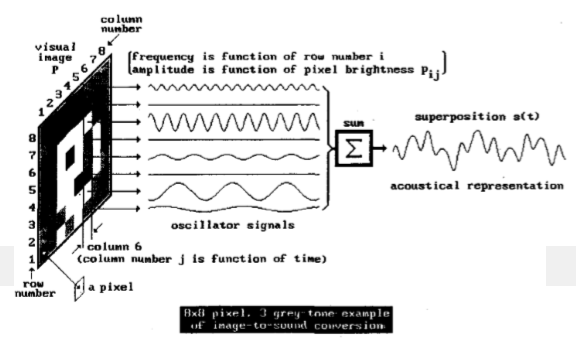
\includegraphics[width=1\textwidth]{image_to_sound}
\caption{\label{fig:image_to_sound} Principles of the image-to-sound mapping \cite{Meijer1992}.}
\end{figure}
  
The experiment showed promising functionality to convert images to sound but lacks a field study test on people with blindness. Moreover, the advantages and disadvantages of this system are yet to be proven. This questions the reliability of the system since there are no recordings of tested data presented in the article of the experiment. However the sound theory represented in the article supports the system's functionality. These theories and the physical setup can be taken into consideration for a system that deals with audiolisation of an image, but the system will have to be tested and evaluated.

\subsection{The Sound of Photographic Image}\label{sec:soundarticle}
A use of images for conversion into sound was performed and described in a paper by Atau Tanaka, who is the chair of digital media and director of culture lab at Newcastle University \cite{Tanaka2012}. The paper describes two processing methods that both convert images into sound.

The first method utilised two image series. The method used to create the sound from the image uses a temporal mapping and additive synthesis on raw grayscale images, by scanning every pixel. Bright pixels produce high notes and a dark pixels produce low notes \cite{Tanaka2012}.

The second method was used for an interactive art installation. The interactive art consisted of a wooden structure with panels covered in rice paper to display Tanaka's pre-processed images from one of the image two series. The images were processed through re-synthesis processes, where the frequency bands were quantisized to whole tones on a pentatonic scale (five notes on a scale) in which the key notes are played one at a time. The image was inverted and each row displayed different frequencies ranging from low to high. An example of this result can be seen in Figure \ref{fig:tanakaresynthesis}. 

\begin{figure}[!h]
\centering
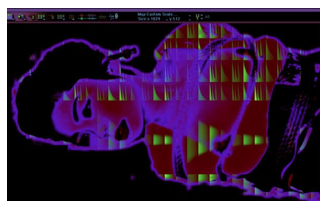
\includegraphics[width=1\textwidth]{tanakaresynthesis}
\caption{\label{fig:tanakaresynthesis}The sounds of Photographic Images second method \cite{Tanaka2012}.}
\end{figure}

To capture human interaction, an infrared camera on top of the installation used viewers' silhouettes as a layer on the negative image which was used to reveal the original black and white image for the viewer, as seen in Figure \ref{fig:tanakainterfacepreview}.

\begin{figure}[!h]
\centering
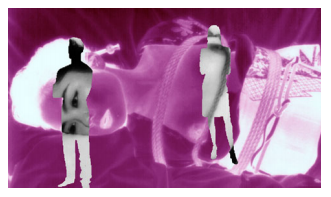
\includegraphics[width=1\textwidth]{tanakainterfacepreview}
\caption{\label{fig:tanakainterfacepreview}Black and white silhouette of the viewer \cite{Tanaka2012}.}
\end{figure}

This interaction also affected the produced sound which were based on the brightness of the processed image and thus produced new sounds. This visualisation of sound through images shows dynamic functionality of a interactive system, which utilises human interaction to alter a preprocessed image. However, since there was no evaluation of this exhibit, it is difficult to know of if the system was a success or inadequate. But due to the system being used in an artistic way, the creator deemed it unnecessary to implement a practical use of this system. A potential use for this system could be in rehabilitation for the lack of motor skills. By using an interface the patient would have to manoeuvre their hands around on an interactive field and have a camera track the movement and give audio feedback to the patient if done right or wrong. Another use could be practising memory for blind people such as an interactive memory game where the user needs to find two equal sounds out of many. 

\section{Methods used to evaluate}\label{sec:methodsusedtoevaluate}

To produce a successful system which utilises signal inputs from an image, the theories for signal processing must be defined and discussed to gain knowledge of different varieties. This section will go through sound analysis.

\subsection{Fourier transform}\label{sub:fourier}

To analyse the effect of a given filter, the Fourier transform can take a given signal and separate the different frequency components in the signal.

\begin{figure}[!h]
\centering
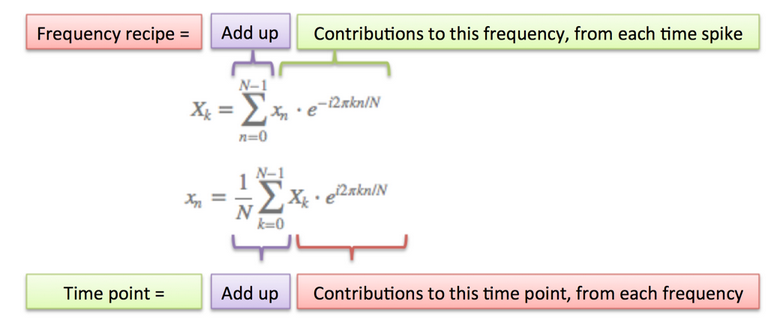
\includegraphics[width=1\textwidth]{MathFourier}
\caption{The mathematical expression of the Fourier transform \cite{MathFourier2013}.}
\end{figure}

The first equation processes the amount of frequency \(k\) at sample \(n\). The equation uses the total number of samples \(N\) and the current sample number \(n\). Thus it uses the expression \(x_n\), which is the value of the signal at sample \(n\), and takes the path of the signal with the speed in radians times \(\frac{n}{N}\). The size, speed and starting angle of a given signal is also defined as amplitude, frequency and phase.      

This process has the benefits of simplifying the signal by separating the important parts such as frequency, which then can be boosted and also neglect unwanted properties.       

\section{State of the art}\label{sec:stateart}
In this project, software that allows images to be converted into sounds are to be considered as the state of the art, as they are closely related to the topic of the project.

\subsection{SonicPhoto}\label{sub:sonic}
SonicPhoto \cite{White2013} is a commercial piece of software developed for Windows that allows a user to input an image and convert it into unique sounds. The software interprets the image as a spectrogram, having pitch on the y-axis and time on the x-axis. The intensity of the pixels is interpreted as the amplitude of the sound. 

\begin{figure}[!h] 
\centering
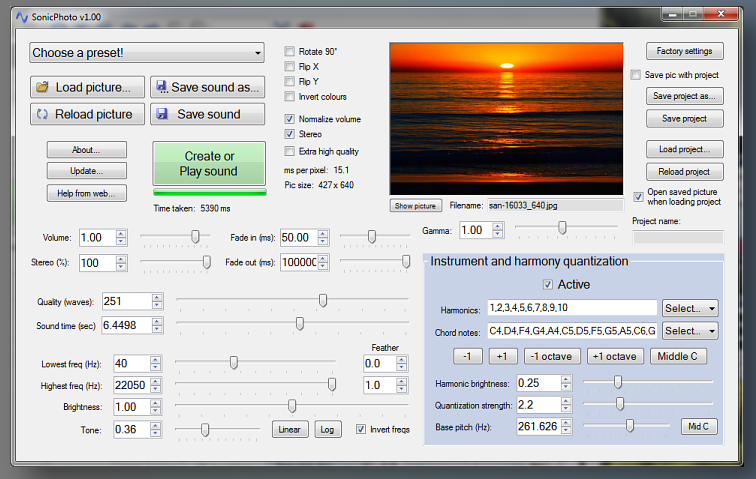
\includegraphics[width=1\textwidth]{sonicphoto}
\caption{\label{fig:sonicphoto} Interface of SonicPhoto \cite{White2013}.}
\end{figure}

The software allows for customisation, such as being able to change the note harmonics, which cord nodes are played, the base of the pitch, and the lowest and highest frequencies. It is also possible to edit the image; changing the alpha channel, rotation, flipping it on the x or y-axis, and inverting the colours. 

\subsection{MetaSynth}\label{sub:metasynth}
MetaSynth, a software for Apple OSX, is also an image-to-sound conversion software. It resembles SonicPhoto by being able to import an image and edit it by for example flipping, rotating, adjusting gamma, and blurring. However, MetaSynth has additional functionality for editing the output sound, as the user can add effects like convolution, grain, delay, reverb, and chorus. The image is interpreted as a spectrogram by the software.

\begin{figure}[!h] 
\centering
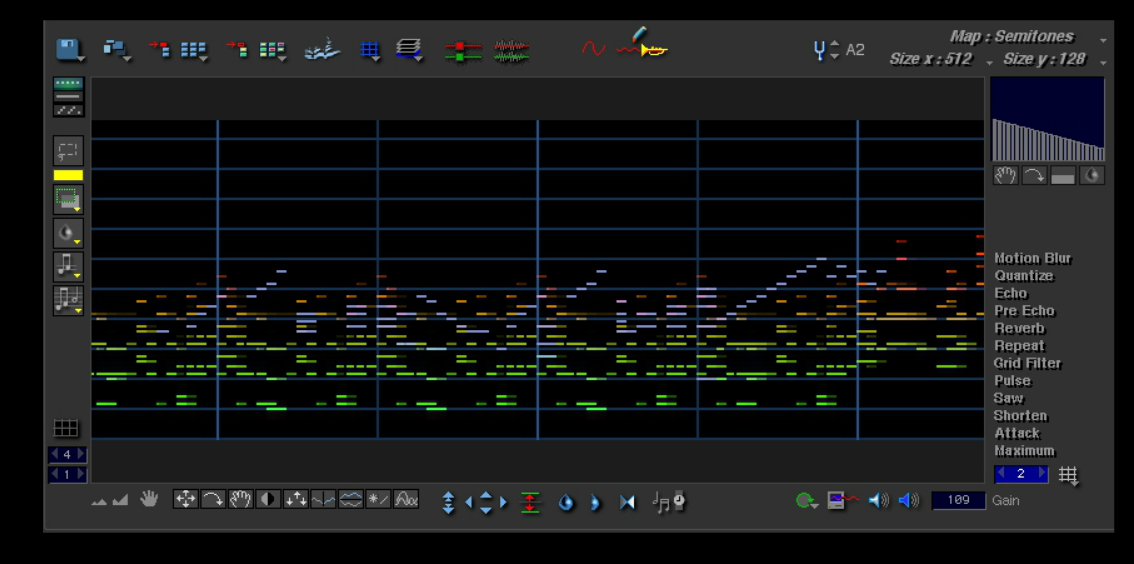
\includegraphics[width=1\textwidth]{metasynth}
\caption{\label{fig:metasynth} Interface of MetaSynth \cite{UISoftware2014}.}
\end{figure}

There is also the possibility to draw freely on an image, while still having all the previously mentioned customisation for both image and sound. In this software, the color of the image determines the stereo placement. Green color for the right stereo, red for the left stereo and yellow in the center. Intensity determines the amplitude. 

Compared to SonicPhoto, MetaSynth emphasises making music in addition to just making sounds. This is because the program allows for adding or putting the audio that the user has created into a sequence to create longer soundtracks.